\documentclass[landscape,twocolumn]{article}
\usepackage{hyperref}
\usepackage{amsmath}
\usepackage{biblatex}
\usepackage{pgfplots}
\usepackage{pgfplotstable}
\addbibresource{references.bib}
\pgfplotsset{compat = 1.17}
\pgfplotstableread[col sep=comma]{results.csv}\results
\title{COMP5329 Assignment 1}
\author{John Hu (zehu4485, 500395897) \and Nicholas Grasevski (ngra5777, 500710654)}
\begin{document}
\maketitle
\begin{abstract}
In this report we implement a multilayer perceptron for a 10 class classification problem. Various deep learning modules are incorporated and tested for this problem, resulting in an architecture with 2 hidden layers which we found to perform best for the classification task.
\end{abstract}

\section{Introduction}
\subsection{Aim}
In this study we aim to compare and contrast the effects of different deep learning modules on the training and validation loss for a simple 10 class classification problem.

\subsection{Background}
Deep learning is an increasingly relevant approach to statistical modelling in order to accurately predict the correct label in a supervised learning setting. According to the universal approximation theorem \cite{universal}, a network with a single hidden layer can approximate any function. This gives neural networks a lot of expressive power.

\section{Methods}
\subsection{Preprocessing}
\subsection{Modules}
\subsubsection{Hidden layer}
\subsubsection{Rectified Linear Unit (ReLU)}
\subsubsection{Weight decay}
\subsubsection{Momentum in Stochastic Gradient Descent (SGD)}
\subsubsection{Dropout}
\subsubsection{Softmax and cross entropy}
\subsubsection{Mini batch training}
\subsubsection{Batch normalization}
\subsection{Design of best model}
\begin{figure}
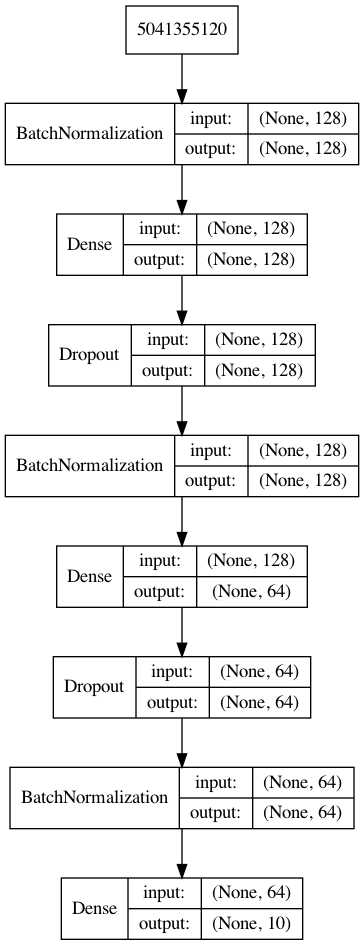
\includegraphics[width=0.5\columnwidth]{model}
\caption{Our best model architecture \label{fig:model}}
\end{figure}

\section{Experiments}
\subsection{Performance}
\subsection{Analysis}
\subsubsection{Hyperparameters}
\subsubsection{Ablation studies}
\subsubsection{Comparison methods}

\section{Results}
\begin{table*}\pgfplotstabletypeset[
    every head row/.style={after row=\hline},
]{\results}\caption{
  Train and test log loss mean and standard deviation on different hyperparameter settings.
  \label{tab:results}
}\end{table*}

\section{Discussion}

\section{Conclusion}

\printbibliography\appendix
\section{Running the code}
\begin{itemize}
\item Dependencies: \texttt{pip install numpy}
\item Usage: \texttt{./assignment1.py}
\end{itemize}
The code assumes the data is stored in a directory called "data". It runs through each of the parameter combinations 5 times and outputs the mean and standard deviation to stdout in csv format. It also logs epoch progress of each run to stderr in json format. The total runtime for running through the 8 combinations 5 times each is about 15 minutes on a Macbook Pro. In order to test architectural changes, the \texttt{model} variable can be modified, it is structured as a list of layers, similar to the keras and pytorch Sequential API. Batch size can also be manually modified in the code, at the cost longer training time.
\end{document}
